\documentclass[11pt]{book}   

%%%%%%%%%%%%%%%%%%%%%%%%%%%%%%%%%%%%%%%%%%%%%%%%%
%%Librerias (este libro se creo usando TEXLIVE)%%
%%%%%%%%%%%%%%%%%%%%%%%%%%%%%%%%%%%%%%%%%%%%%%%%%
      
\usepackage[utf8]{inputenc}
\usepackage[spanish]{babel}

\usepackage{hyperref}

\usepackage{appendix}
\usepackage{makeidx}

\usepackage[toc,style=long3colheaderborder,footnote,acronym]{glossaries} 
\usepackage{fancyhdr}
\usepackage{showidx}
\usepackage{listings}
\usepackage{color}
\usepackage{graphicx}
\usepackage{float}
\usepackage{wrapfig}
\usepackage{enumerate}

\definecolor{dkgreen}{rgb}{0,0.6,0}
\definecolor{gray}{rgb}{0.5,0.5,0.5}
\definecolor{mauve}{rgb}{0.58,0,0.82}

%%%%%%%%%%%%%%%%%%%%%%%%%%%%%%%%%%%%%%%%%%%%%%%%%%%%%%%%%%%
%%Definiendo los atributos para el codigo de programacion%%
%%%%%%%%%%%%%%%%%%%%%%%%%%%%%%%%%%%%%%%%%%%%%%%%%%%%%%%%%%%

\lstset{frame=tb,
  language=Java,
  aboveskip=3mm,
  belowskip=3mm,
  showstringspaces=false,
  columns=flexible,
  basicstyle={\small\ttfamily},
  numbers=none,
  numberstyle=\tiny\color{gray},
  keywordstyle=\color{blue},
  commentstyle=\color{dkgreen},
  stringstyle=\color{mauve},  
  breaklines=true,
  breakatwhitespace=true
  tabsize=3
}

\makeglossary
\makeindex
\parindent0pt  \parskip10pt             

%%%%%%%%%%%%%%%%%%%%%%%%%
%%Entradas del glosario%%
%%%%%%%%%%%%%%%%%%%%%%%%%


\newglossaryentry{AppStores}
{
	name={App Store},
	description={Forma corta en ingles de las palabras \textit{Applicaction Store} que significa en español 		tienda de aplicaciones. Una AppStore suele ser un 			entorno virtual en el cual los usuarios de un 				determinado sistema operativo móvil (Android, IOS, 			Symbian, etc.) pueden comprar, descargar e instalar 		programas para su dispositivo móvil.}
}

\newglossaryentry{Angry Birds}
{
	name={Angry Birds},
	description={En español \textit{Pájaros Furiosos}, es un Videojuego creado en 2009 por la empresa finlandesa Rovio Mobile el cual a acumulado más de mil millones de descargas en diferentes plataformas móviles como lo son IOS, Android y Symbian.}
}

\newglossaryentry{Smartphone}
{
	name={smartphone},
	description={En español \textit{Teléfono inteligente}, es un teléfono móvil construido sobre una plataforma informática móvil, con una mayor capacidad de computación y conectividad que un teléfono móvil convencional, se le dice inteligente por su capacidad de procesar datos complejos sin necesidad de un computador externo.}
}

\newglossaryentry{PDA}
{
	name={PDA},
	description={Acrónimo de las palabras en ingles \textit{personal digital assistant} que en español se traduce \textit{asistente digital personal}, es un computador de mano diseñado para superar la agenda electrónica proveyendo más servicios para el día a día como lo son el calendario, lista de contactos, bloc de notas y recordatorios, siendo uno de los primeros dispositivos táctiles vendidos en el mercado se popularizo mucho pero con el paso del tiempo fue remplazado por los celulares de alta gama.}
}

\newglossaryentry{Beeper}
{
	name={beeper},
	description={Llamado en español \textit{mensáfono}, es un dispositivo móvil muy simple que recibe mensajes de texto cortos, usado para contactar a personas que se movilizaban mucho en caso de emergencia.}
}

\newglossaryentry{Handie Talkie}
{
	name={Handie Talkie},
	description={Nombre completo \textit{Handie Talkie H12-16}, fue el primer dispositivo móvil creado para comunicar tropas en la segunda guerra mundial cuya banda de frecuencias en ese tiempo no superaban los 600 kHz.}
}
%%%%%%%%%%%%%%%%%%%%%%%%%%%%%%%%%%%%%%%%%%%%%%%%%%%%%%%%%%%%
%%Inicio del Libro										  %%
%% Note que el formato para libro es especial y por ende  %%
%% las paginas aparecerean un poco ajustadas en la margen %%
%% para cuestiones de impresion.                          %%
%%%%%%%%%%%%%%%%%%%%%%%%%%%%%%%%%%%%%%%%%%%%%%%%%%%%%%%%%%%%

\title{\bf Mi Primera Aplicación En Android\\ MAEOCS\\ Un Ejemplo Nada Más}    % Supply information
\author{Carlos I. Gaitán M., Edward H. Jiménez M.}              %   for the title page.
\date{\today}                           % Use current date. 
\begin{document}                        
\frontmatter                            % only in book class 
\maketitle                              % Print title page.
\tableofcontents                        % Print table of contents
\mainmatter                             % only in book class 


%%%%%%%%%%%%%%%%%%%%%%%
%%Parte 1, Capitulo 1%%
%%%%%%%%%%%%%%%%%%%%%%%

\part{El mundo móvil y Android}  
    
\chapter{¿Por qué una aplicación móvil?}

\newpage
\section{El mundo móvil}              	
Hoy en día es muy común escuchar acerca de los dispositivos móviles y las aplicaciones que existen para estos, pero cuantas veces nos hemos detenido a pensar por un momento como en realidad funciona este mundo (que no es tan nuevo como muchos pensarían) y que tan fácil es entrar en su mercado, creando aplicaciones móviles o juegos para venderlos en las famosas \gls{AppStores}. A lo largo de este capitulo expondremos los beneficios de entrar al mundo móvil y sus ventajas competitivas frente al mercado que viene, para ello empezaremos con enumerar algunas de sus ventajas:

\begin{itemize}
\item La cifra de usuarios móviles en el mundo esta al rededor del 85\% de la población mundial.
\item Esta constantemente conectado.
\item Si juntamos el tiempo de juego de todos los usuarios de \gls{Angry Birds} se suman 205,343 años.
\item Siempre esta cerca de la persona.
\item Tiene canales de pago exclusivos y seguros (\gls{AppStores}).
\item Contiene la información personal de acceso sencillo.
\item Captura el concepto social del consumismo.
\end{itemize}

Los dispositivos móviles siempre han sido un instrumento que representa portabilidad, eficacia, conectividad, privacidad y agilidad para las personas que hacen uso de sus múltiples capacidades creando así un publico bastante grande que hace uso de estos dispositivos ya sea para jugar, trabajar o simplemente comunicarse. Sabia usted que hoy en día existen más lineas telefónicas móviles que fijas y las personas que poseen un dispositivo móvil pasan más del 80\% del tiempo con este al lado, sabia que en Colombia el número de lineas móviles \ref{fig:estadisticas2} es más de seis veces el número de lineas fijas \ref{fig:estadisticas1}; esto, sin duda, nos hace pensar acerca del increíble cubrimiento que puede llegar a tener una aplicación como lo puede ser un gestor de correo, un gestor de actividades, una agenda virtual, etc.

%%%%%%%%%%%%%%%%%%%%%%%%%%
%%Imagen de estadisticas%%
%%%%%%%%%%%%%%%%%%%%%%%%%%
\newpage
\begin{figure}[H]
  \centering
    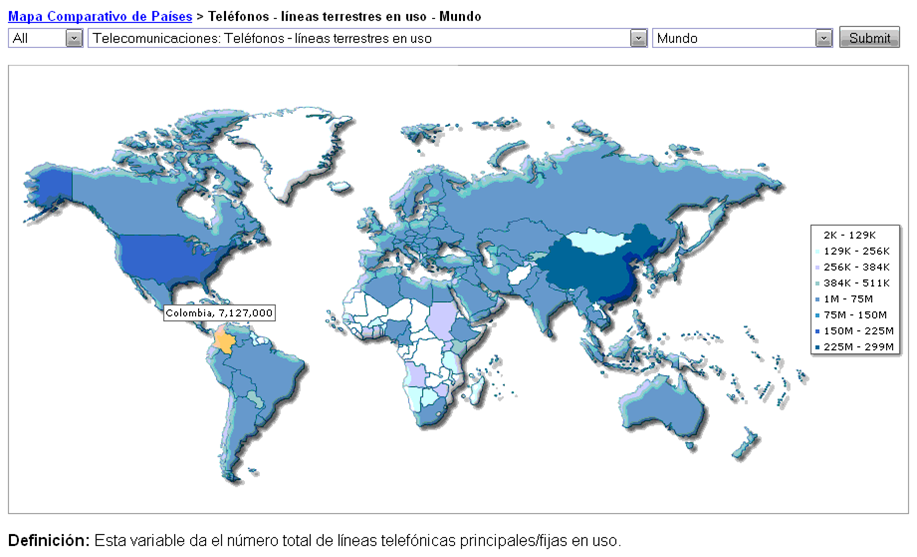
\includegraphics[width=1.0\textwidth]{estadisticas_1}
  \caption{Estadísticas lineas fijas en Colombia}
  \label{fig:estadisticas1}
\end{figure}

\begin{figure}[H]
  \centering
    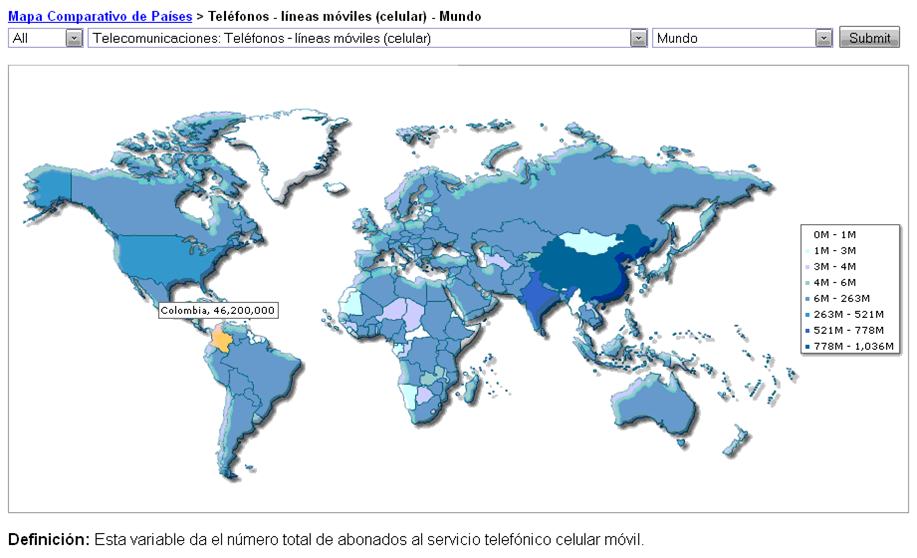
\includegraphics[width=1.0\textwidth]{estadisticas_2}
  \caption{Estadísticas lineas móviles en Colombia}
  \label{fig:estadisticas2}
\end{figure}

\section{La historia del mundo móvil}
Esta sección queremos iniciarla con la frase \textit{"para saber a donde vas tienes que saber de donde vienes"}, en el mundo móvil si que es importante conocer de donde viene no solo la tecnología sino también las aplicaciones que queremos llegar a diseñar por eso en este capitulo profundizaremos un poco de lo que fue e incluso aun sigue siendo.

%%%%%%%%%%%%%%%%%%%%%%%%%%%%
%%Figura al lado del texto%%
%%%%%%%%%%%%%%%%%%%%%%%%%%%%

\begin{wrapfigure}{r}{0.5\textwidth}
  \vspace{-20pt}
  \begin{center}
    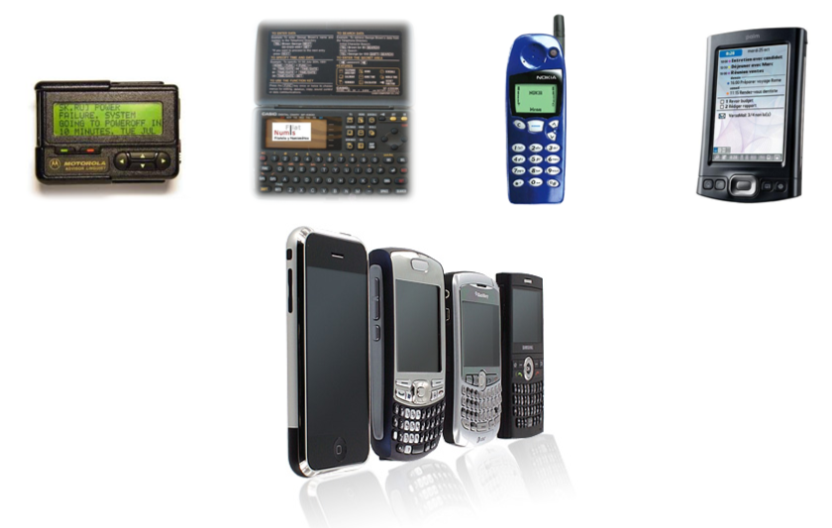
\includegraphics[width=0.48\textwidth]{historia_1}
  \end{center}
  \vspace{-20pt}
  \caption{Cuadro de dispositivos móviles}
  \label{fig:historia_1}
  \vspace{-10pt}
\end{wrapfigure}

Muchas personas suelen pensar que la movilidad comienza y termina con los celulares pero la verdad es que detrás de los celulares viene todo un mundo de dispositivos como los asistentes digitales (\gls{PDA}), el \gls{Beeper} o las agendas electrónicas que fueron en realidad los que fusionados con los celulares dieron nacimiento a los \gls{Smartphone}.

Hagamos una pequeña reseña histórica de los dispositivos móviles; como todo avance tecnológico comienza con una necesidad o en este caso dos: la capacidad de permanecer conectado y poder organizar grandes cantidades de información a cualquier hora del día en el lugar donde que me encuentre (la casa, el trabajo, la calle, el bus, etc.), normalmente este tipo de necesidades las imponían compañías e importantes empresarios a las empresas de telecomunicaciones las cuales respondieron no a los empresarios sino a las fuerzas armadas de la segunda guerra mundial con el \gls{Handie Talkie}, años después comenzó la creación de los primeros teléfonos móviles para el publico con pesos aproximados a un kilogramo y con un precio promedio de cuatro mil dolares, con el tiempo hubo respuestas más baratas para los empresarios pequeños como lo es el \gls{Beeper} y mucho después atendiendo a la segunda necesidad nacen las agendas electrónicas las cuales serian rápidamente remplazadas por los \gls{PDA} que al final terminarían fusionándose con los teléfonos móviles para suplir las dos necesidades como una sola.

Lo más importante para destacar no es el avance ni los cambios tecnológicos que ha tenido el mundo móvil, por el contrario lo que vale la pena evaluar es lo genérico y convencional que se han mantenido sus aplicaciones básicas como lo son el calendario, la agenda de contactos, la calculadora, la agenda de tareas y claro no pueden faltar los juegos, si hay algún cambio que atribuir a lo mencionado anteriormente es sobre la usabilidad y calidad de imagen lo cual quiere decir de una u otra forma que si se crean las mismas aplicaciones más amigables y con mejor calidad de imagen sin duda alguna remplazaran a las que vienen pre-instaladas en el dispositivo.

\section{Los grandes de hoy en día}
Vale la pena aclarar desde un inicio que con grandes no nos referimos ni al tamño de la compañia ni a la tecnologia en los dispositivos o sistemas operativos, con "grandes" hacemos referencia a los más usados en el mercado hoy en día y para ello nos apoyamos en dos gráficas: mercado de los sistemas operativos en el mundo \ref{fig:estadisticas4} y en colombia \ref{fig:estadisticas3}.

%%%%%%%%%%%%%%%%%%%%%%%%%%
%%Imagen de estadisticas%%
%%%%%%%%%%%%%%%%%%%%%%%%%%

\begin{figure}[H]
  \centering
    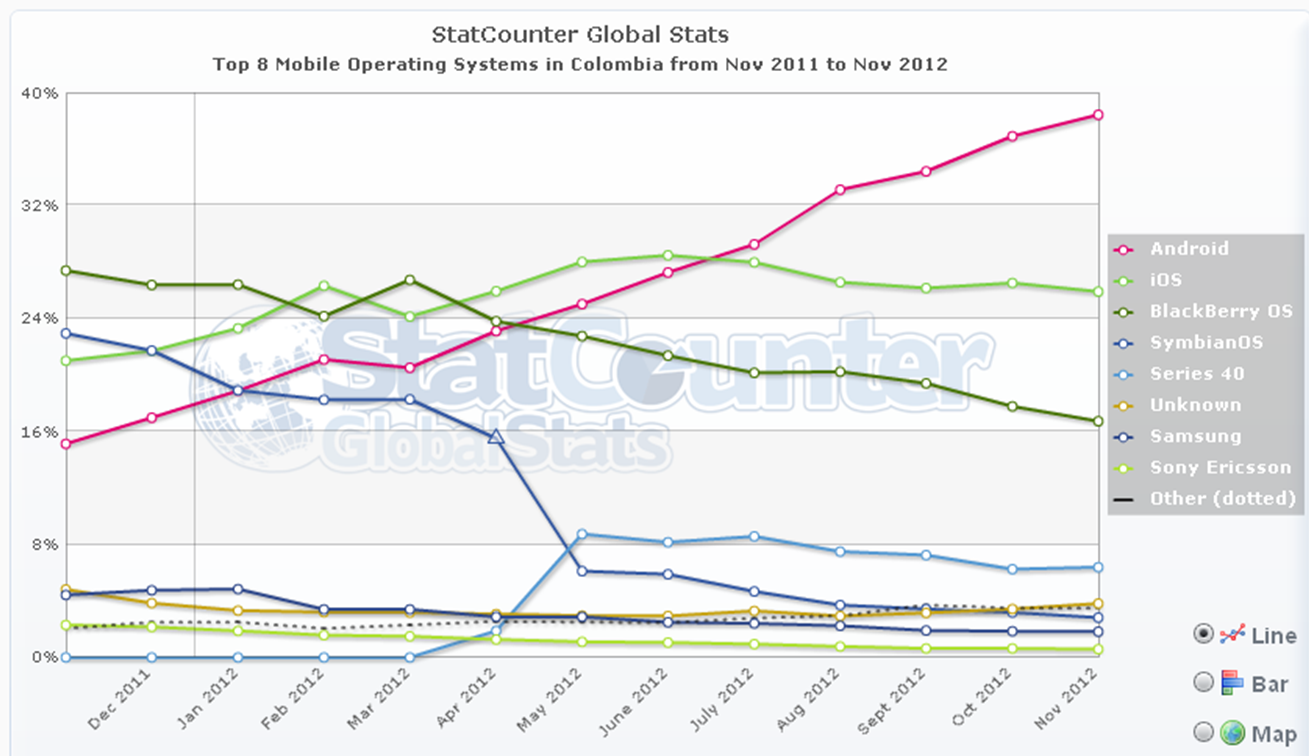
\includegraphics[width=1.0\textwidth]{estadisticas_3}
  \caption{Estadísticas sistemas operativos móviles en Colombia}
  \label{fig:estadisticas3}
\end{figure}

\begin{figure}[H]
  \centering
    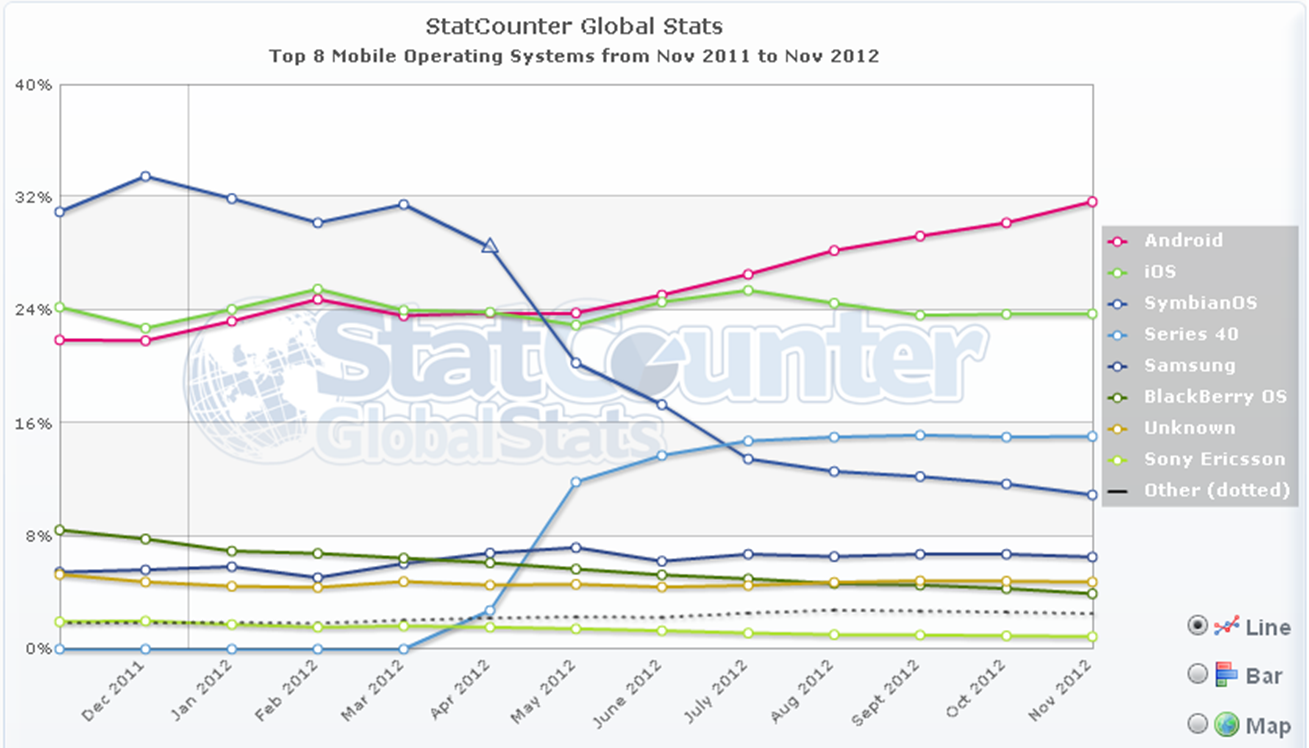
\includegraphics[width=1.0\textwidth]{estadisticas_4}
  \caption{Estadísticas sistemas operativos móviles en el mundo}
  \label{fig:estadisticas4}
\end{figure}

Como se puede apreciar en las gráficas vale la pena hablar de cuatro grandes:

\begin{itemize}
\item Symbian: Es un sistema operativo móvil que si bien hoy en día ya no esta en el mercado hasta hace poco fue uno de los más usados por los \gls{Smartphone}, fue creado en convenio por muchas compañías como Nokia, Sony Mobile Communications, Psion, Samsung, Siemens, Arima, Benq, Fujitsu, Lenovo, LG, Motorola, Mitsubishi Electric, Panasonic, Sharp, etc. Durante todo su ciclo fue siendo comprado lentamente por Nokia hasta que este se apodero totalmente de el, con el tiempo y siendo Nokia una de las empresas más imponentes en celulares Symbian gano un gran publico el cual lentamente fue desapareciendo en el tiempo, todo el mundo sabe que Symbian marco el inicio de los sistemas operativos para \gls{Smartphone} pero para 2012 lo único que marco fue el final de su era, muchos atribuyen su desaparición a la falta de avances y otros más a su falta de publicidad como sistema operativo, una ultima teoría bastante valida se atribuye a la falta de aplicaciones móviles que pudieran competir con las de su competencia.

\item Blackberry: BlackBerry OS es un sistema operativo móvil desarrollado por Research In Motion para sus dispositivos BlackBerry. El sistema operativo de Blackberry fue creado para uso empresarial y asi fue que se hizo famoso sin embargo cuando salio al mercado para el publico en general fue bien recibido por sus dos grandes ventajas: el servicio de mensajería y su impresionante seguridad la cual traía del mercado empresarial del cual había aprendido tanto, actualmente Blacberry como sistema operativo y como teléfono móvil esta pasando por una crisis pues se ha visto arrinconado frente a su competencia por razones muy similares a las de Symbian pero la razón más grande que lo ha venido dejando a bajo frente a Android y IOS es la constante queja de muchos de sus usuarios frente a la usabilidad y lo rígido del sistema.

\item Android: Es un sistema operativo móvil basado en Linux, que junto con un conjunto de aplicaciones da una oferta libre para el mundo móvil. Fue desarrollado inicialmente por Android Inc., una firma comprada por Google en 2005. En sus inicios Android fue una revolución para aquellos que siempre han buscado el software libre y gratuito siendo así el sistema operativo con más aplicaciones gratis en su \gls{AppStores}, a diferencia de muchos de los sistemas operativos móviles no esta ligado a una marca de teléfono en especifico sin embargo la tabla de dispositivos que soporta no es tan grande como muchos desearíamos, es un sistema operativo que a cada día tiene más usuarios y esto se debe a su interfaz fácilmente adaptable a los gustos de los usuarios y también a su gran cantidad de aplicaciones no solo para su \gls{AppStores} sino también en diferentes paginas o sitios web.

\item IOS: Es un sistema operativo móvil de Apple. Originalmente desarrollado para el iPhone, siendo después usado en dispositivos como el iPod Touch, iPad y el Apple TV. Una gran desventaja y fuerte de IOS que le ha costado muchos usuarios es lo cerrado de su sistema y el poco entusiasmo o facilidades que da a los programadores para desarrollar para su plataforma; provocando asi que solo se pueda usar en dispositivos Apple con aplicaciones en su mayoría desarrolladas por empresas colocando a IOS como la plataforma con las aplicaciones más costosos en el mercado móvil.

\end{itemize}

\newpage
\section{El mercado móvil} 
Aunque no profundizaremos mucho en esta sección si nos parece muy importante que haya una clara orientación de como es el mercado al que vamos a entrar y como pueden vender sus aplicaciones.

\begin{itemize}

\item Aplicativos con costo: Esta opción hace referencia a cobrar directamente la aplicación en la \gls{AppStores}, en este caso hay que tener mucho cuidado pues el precio que pongamos puede hacer a nuestra aplicación un gran éxito o un gran fracaso para ello se debe considerar tres cosas:
	\begin{itemize}
	\item Costo promedio de la tienda: Costo al que están la mayoría de las aplicaciones del mismo estilo que la que intenta vender.
	\item Costo/periodo de la suscripción a la \gls{AppStores}: Toda tienda cobra un periodo suscripción para poder subir las aplicaciones a la tienda.
	\item Porcentaje de ganancia real sobre la aplicación: Adicional al costo de suscripción la tienda también impone un porcentaje de ganancia sobre nuestras aplicaciones.
	\end{itemize}
\item Aplicativos sin costo: Esta opción hace referencia a dejar gratis nuestra aplicación en la \gls{AppStores}, en este caso hay dos opciones si nuestro interés es hacer algo de dinero:
	\begin{itemize}
	\item Publicidad: Esta opción consiste en activar opciones publicitarias para nuestra aplicación permitiendo a la tienda insertar contenidos adicionales los cuales nos pagaran dependiendo de la cantidad de descargas y usos de la aplicación, para usar esta opción debemos tener claro que la usaremos desde el inicio de la creación de nuestra aplicación.
	\item Adicionales: Una estrategia muy común en las aplicaciones móviles es liberar el core o aplicación base completamente gratis y cobrar adicionales, un ejemplo claro son los juegos donde un arma mejor o personalizar a tu personaje puede costarte unos cuantos centavos. Para esta opción las tiendas disponen de sistemas especiales que debes integrar a tu aplicación desde que comienzas a desarrollarla.
	\end{itemize}

\end{itemize}

\chapter{¿Por Qué Una Aplicación en Android?}  
\newpage
\section{La historia de Android}
blablablabla
\section{Ventajas y desventajas de Android}
blablablabla
\section{Android en el mundo}                 
blablablabla
\section{Android en el mercado móvil} 
blablablabla

\chapter{Consejos útiles}  
blablablabla
\section{Provectos móviles}
blablablabla
\section{Wireframes}                 
blablablabla


\part{Conociendo Android}    
            
\chapter{Preparándolo todo}              
\newpage
\section{El SDK de Android}
Es importante aclarar que desde este punto el libro tomara una orientación de guía, ayudando a aclarar desde como instalar todo lo que necesitamos para instalar el ambiente para desarrollar hasta como crear cierto tipo de aplicaciones, para que la guía sea lo más útil debe prestar especial atención a las áreas resaltadas o sombreadas de las imágenes. 

Conseguir e instalar el SDK:

\begin{enumerate}[1.]

\item Lo primero es ir a la pagina de Android y descargar todo lo que necesitamos (\href{http://developer.android.com/sdk/index.html}{http://developer.android.com/sdk/index.html}).

\begin{figure}[H]
  \centering
    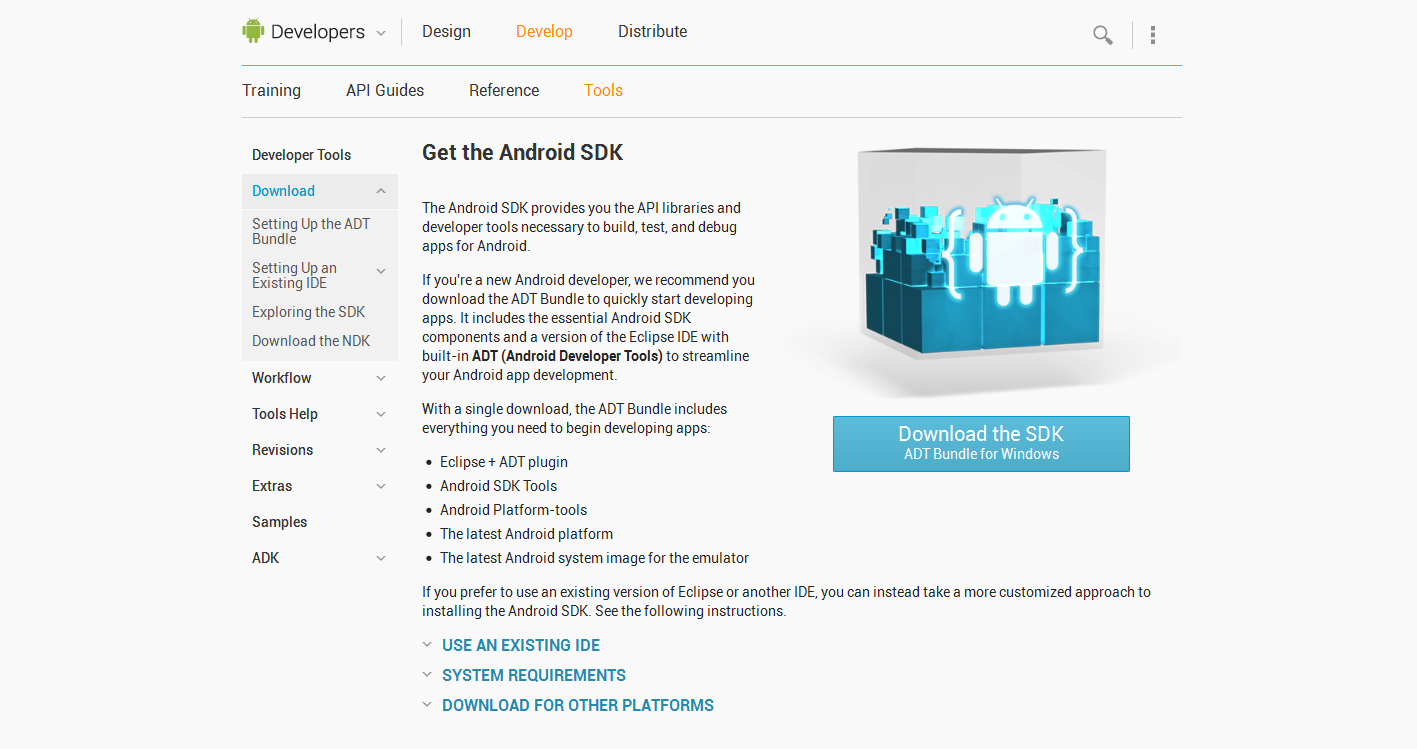
\includegraphics[width=1.0\textwidth]{tutorial_3}
  \caption{Pagina principal del SDK Android 2012}
  \label{fig:tutorial_3}
\end{figure}
\newpage
\item Lea detenidamente los términos de la licencia y a continuación seleccione aceptar los términos y la casilla siguiente de acuerdo a la arquitectura de su sistema operativo, al dar clic en el botón de descargas comenzara a descargarse un paquete comprimido que contiene el SDK y un eclipse listo para empezar a desarrollar.

\begin{figure}[H]
  \centering
    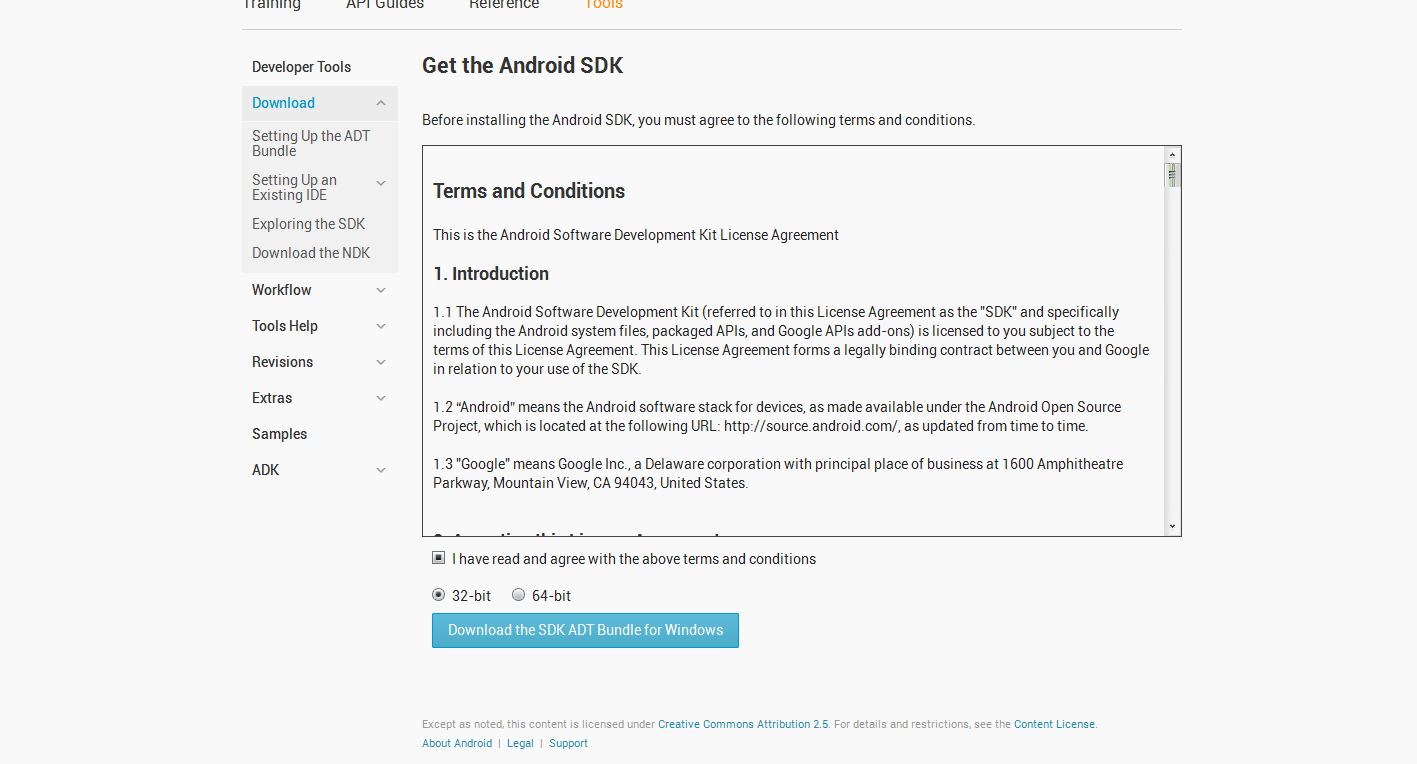
\includegraphics[width=1.0\textwidth]{tutorial_4}
  \caption{Términos de contrato}
  \label{fig:tutorial_4}
\end{figure}
\newpage
\item Descomprima el paquete y a continuación abra la carpeta que dice eclipse y ejecute el entorno, como sugerencia personal mantenga este entorno unicamente para cuando vaya a programar en Android.

\begin{figure}[H]
  \centering
    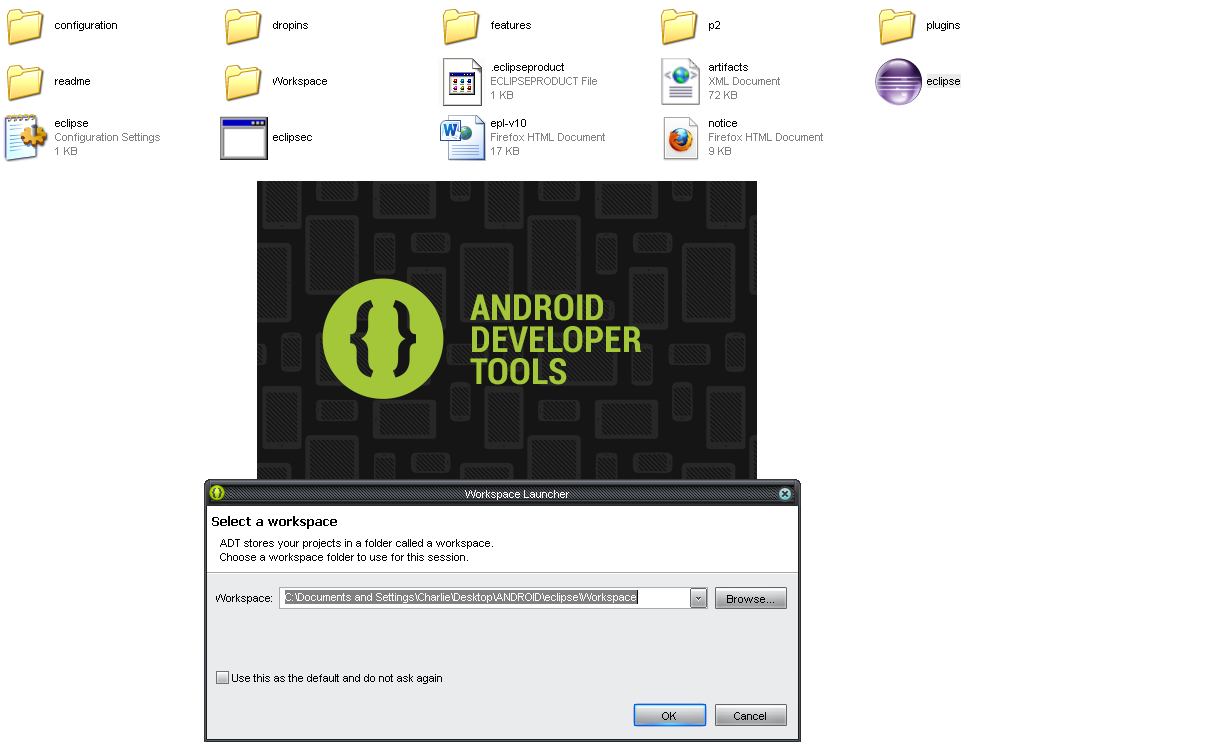
\includegraphics[width=1.0\textwidth]{tutorial_7}
  \caption{Carpeta de eclipse}
  \label{fig:tutorial_7}
\end{figure}
\newpage
\item En la barra de arriba aparece un icono de Android con una flecha hacia abajo, este icono simboliza el SDK Manager el cual sera nuestro gestor de paquetes y versiones de Android, a continuación dar clic en el SDK Manager.

\begin{figure}[H]
  \centering
    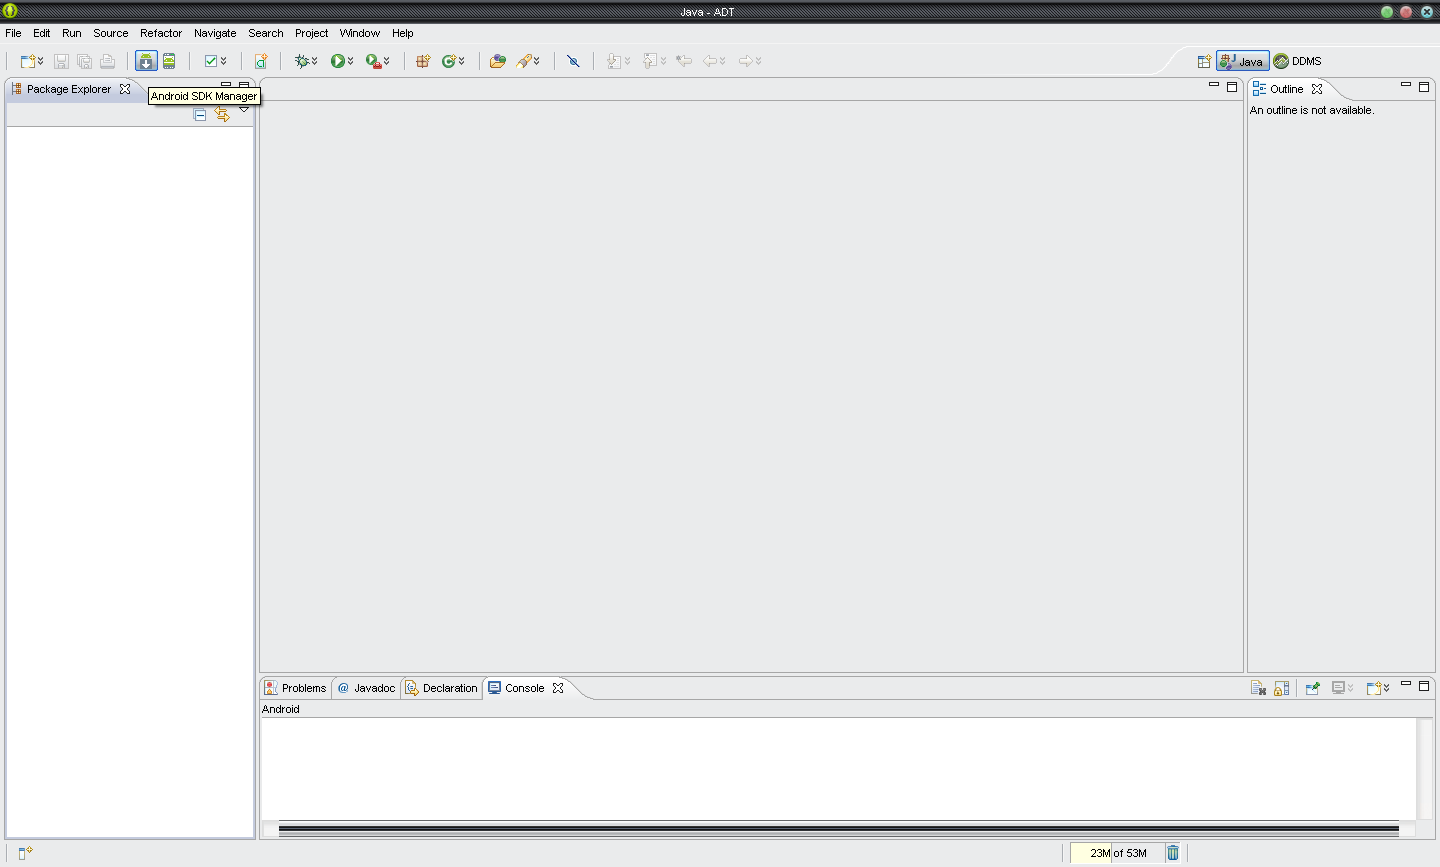
\includegraphics[width=1.0\textwidth]{tutorial_8}
  \caption{Entorno de eclipse para Android}
  \label{fig:tutorial_8}
\end{figure}
\newpage
\item Veremos una lista de paquetes separados por las versiones existentes de Android, en esta parte trabajaremos con la versión 2.3.3 por lo tanto sugerimos seleccionar los mismos paquetes que aparecen en la imagen, al dar clic en instalar debemos estar consientes de que estos paquetes pueden llegar a ser bastante pesados y que dependiendo de nuestra conexión a Internet y otros factores la instalación puede tomar horas.

\begin{figure}[H]
  \centering
    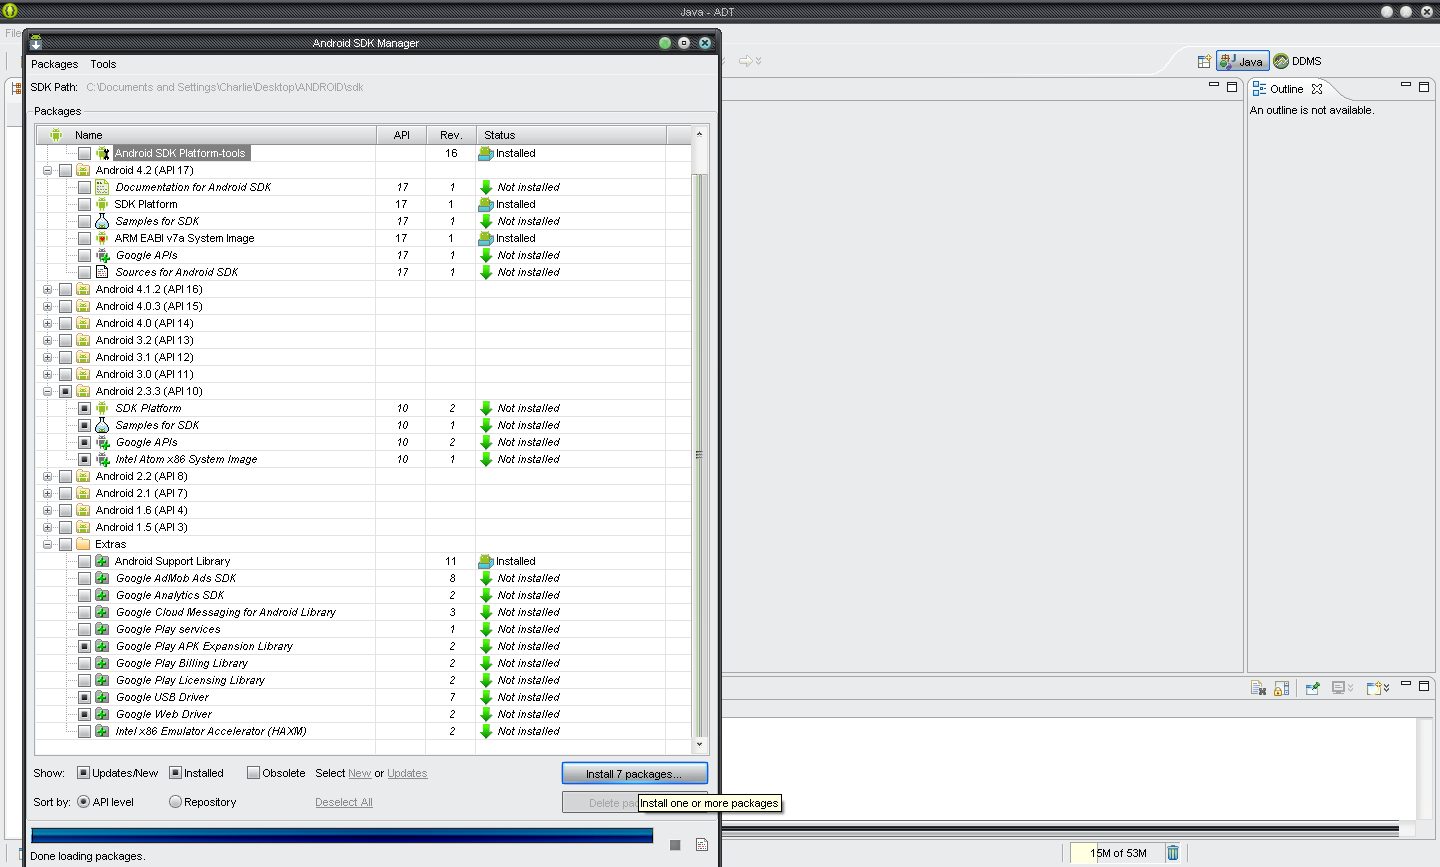
\includegraphics[width=1.0\textwidth]{tutorial_9}
  \caption{SDK Manager de Android}
  \label{fig:tutorial_9}
\end{figure}
\end{enumerate}

\newpage
\chapter{Mi primera actividad}              
\newpage
\section{Creando un proyecto Android}
A partir de aquí evitaremos las imágenes de pantalla en lo posible pues más que una guía visual del entorno de eclipse para Android lo que buscamos es una guía conceptual del código y el desarrollo en Android.

\begin{enumerate}[1.]

\item Crear un proyecto Android es muy similar a como se hace para Java en eclipse, basta con hacer clic secundario en el área de exploración de proyectos y seleccionar la opción de un nuevo proyecto Android.

\begin{figure}[H]
  \centering
    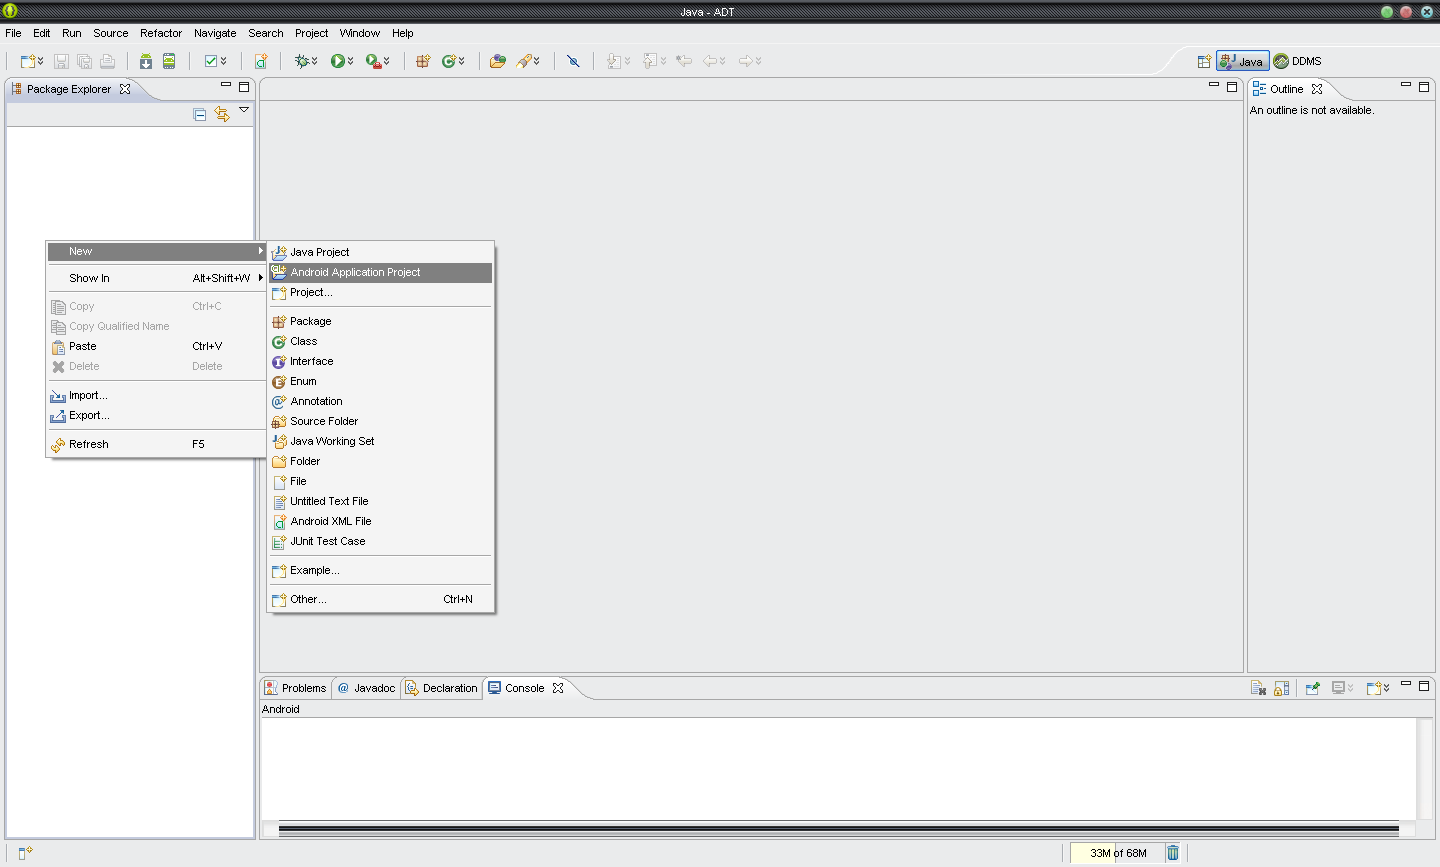
\includegraphics[width=1.0\textwidth]{tutorial_19}
  \caption{Creando un nuevo proyecto Android}
  \label{fig:tutorial_19}
\end{figure}

\newpage
\item Para el nuevo proyecto tenemos varias opciones la primera hace referencia al nombre que queremos aparezca en el dispositivo en la segunda el nombre del proyecto en eclipse, la tercera es para los paquetes sobre los que se desarrollara el proyecto y las ultimas a las versiones sobre las cuales se ejecutara el proyecto.

\begin{figure}[H]
  \centering
    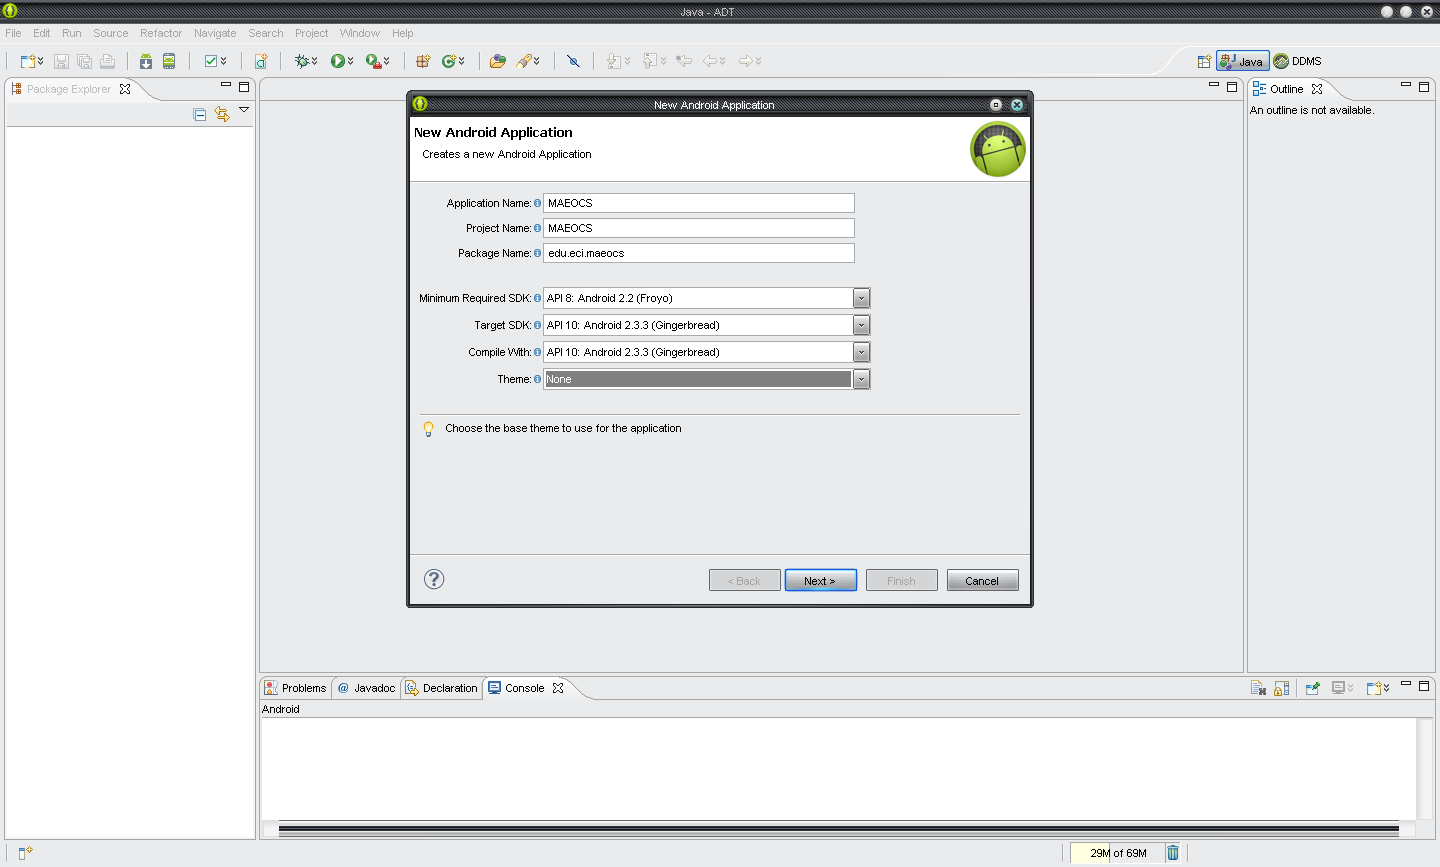
\includegraphics[width=1.0\textwidth]{tutorial_20}
  \caption{Ventana de nuevo proyecto}
  \label{fig:tutorial_20}
\end{figure}

\newpage
\item La siguiente parte es para seleccionar el icono que aparecerá en nuestra aplicación, Android nos provee con algunas opciones estándar, pero si diseñamos nuestros propios iconos podemos seleccionarlos en la pestaña de imágenes, en este ultimo caso debemos tener cuidado con los tamaños de la imagen para obtener la mejor calidad posible dependiendo del tamaño del dispositivo que vaya a usar nuestra aplicación.

\begin{figure}[H]
  \centering
    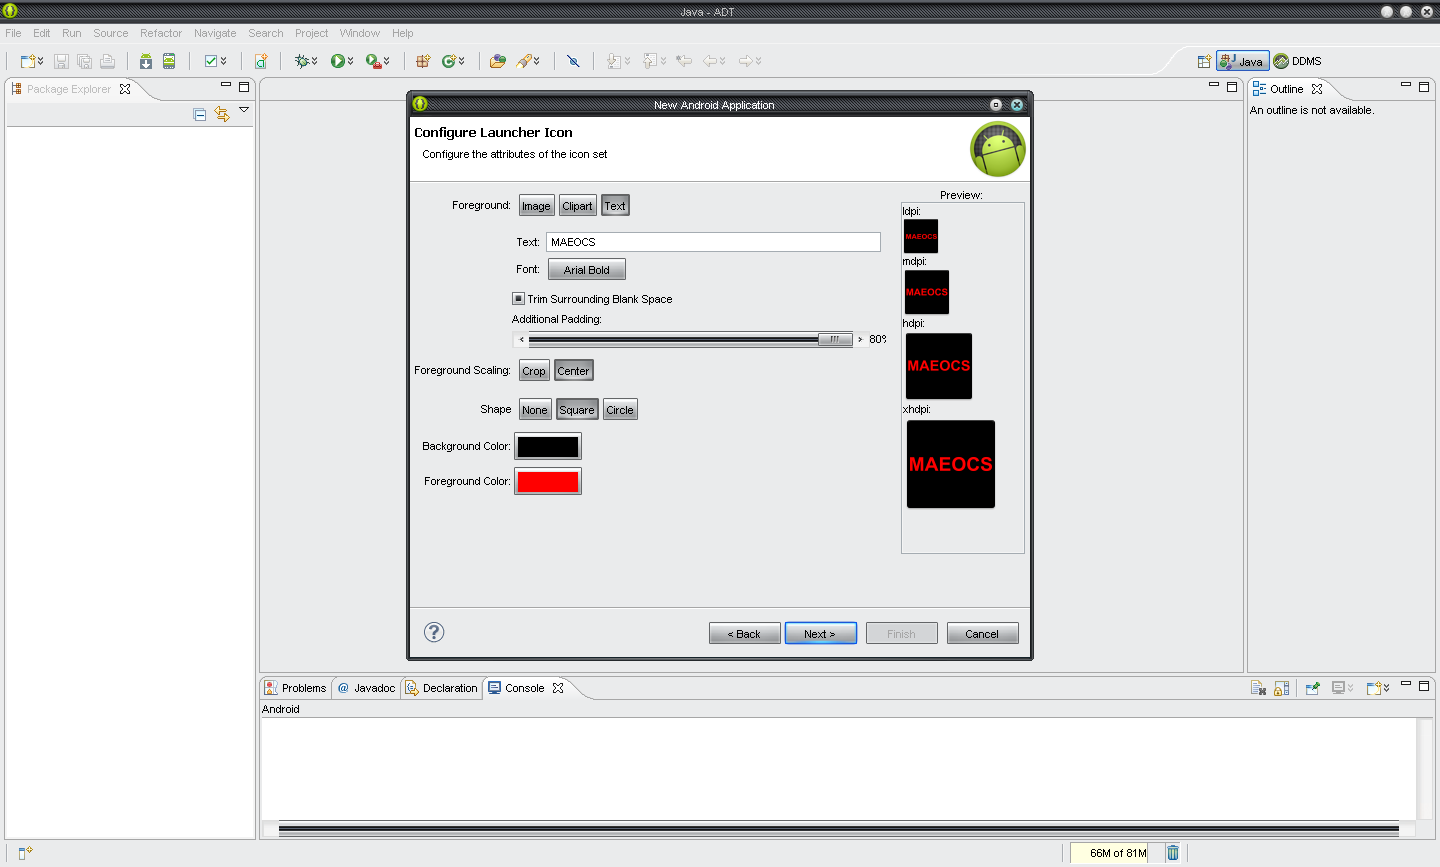
\includegraphics[width=1.0\textwidth]{tutorial_21}
  \caption{Seleccionando el icono de la aplicación}
  \label{fig:tutorial_21}
\end{figure}
\newpage
\item La siguiente ventana corresponde a la selección del tipo de actividad que vamos a crear, como trabajaremos en la versión 2.3.3 el tipo de actividad solo puede ser blanca ya que las otras opciones corresponden a versiones superiores.

\begin{figure}[H]
  \centering
    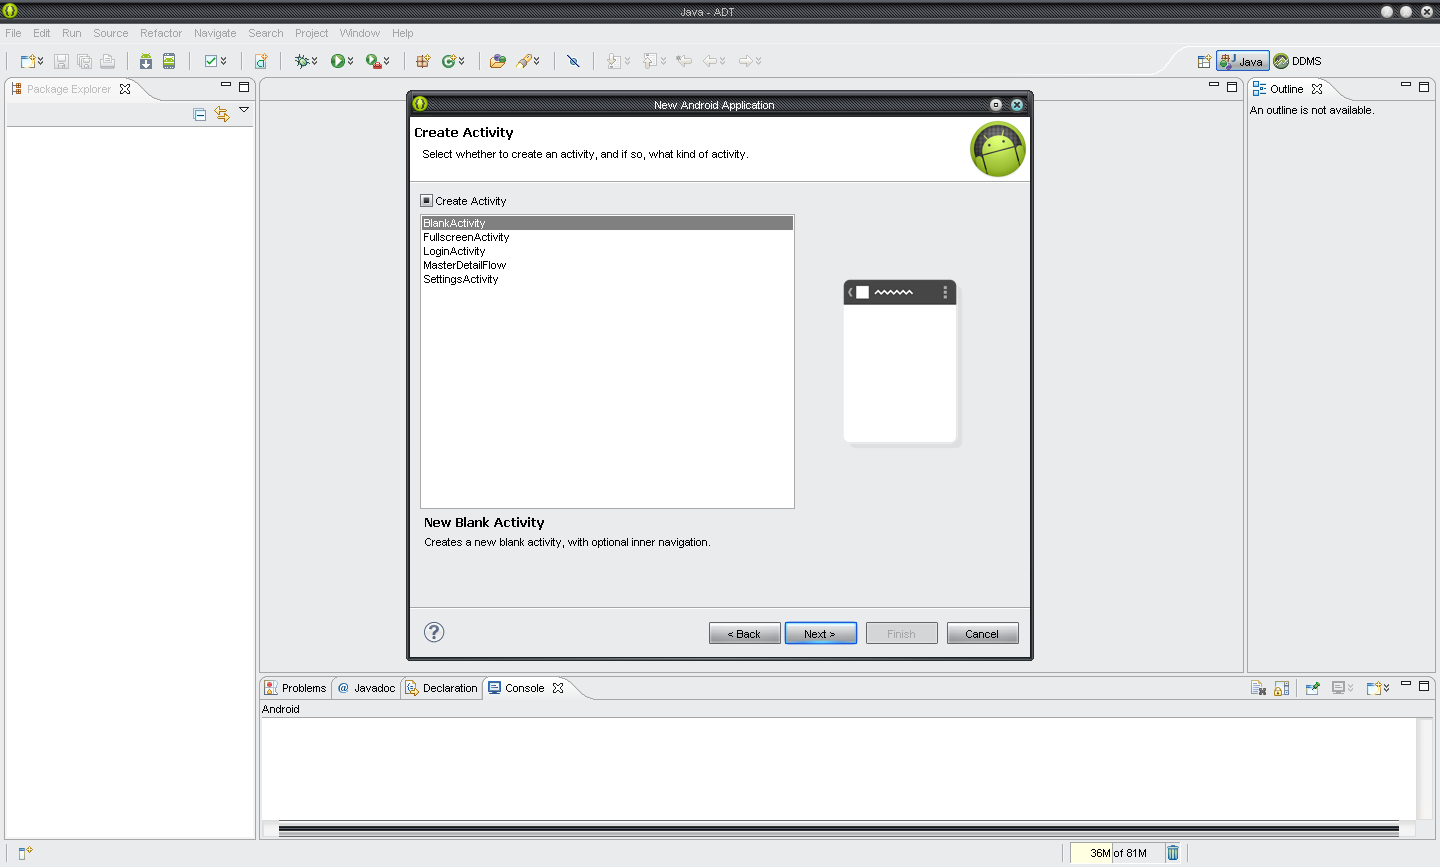
\includegraphics[width=1.0\textwidth]{tutorial_22}
  \caption{Términos de contrato}
  \label{fig:tutorial_22}
\end{figure}
\newpage
\item Por ultimo debemos nombrar la actividad y la interfaz principales que acabamos de crear, si deseamos que la actividad principal sea otra clase diferente debemos especificarlo más adelante en el manifiesto.

\begin{figure}[H]
  \centering
    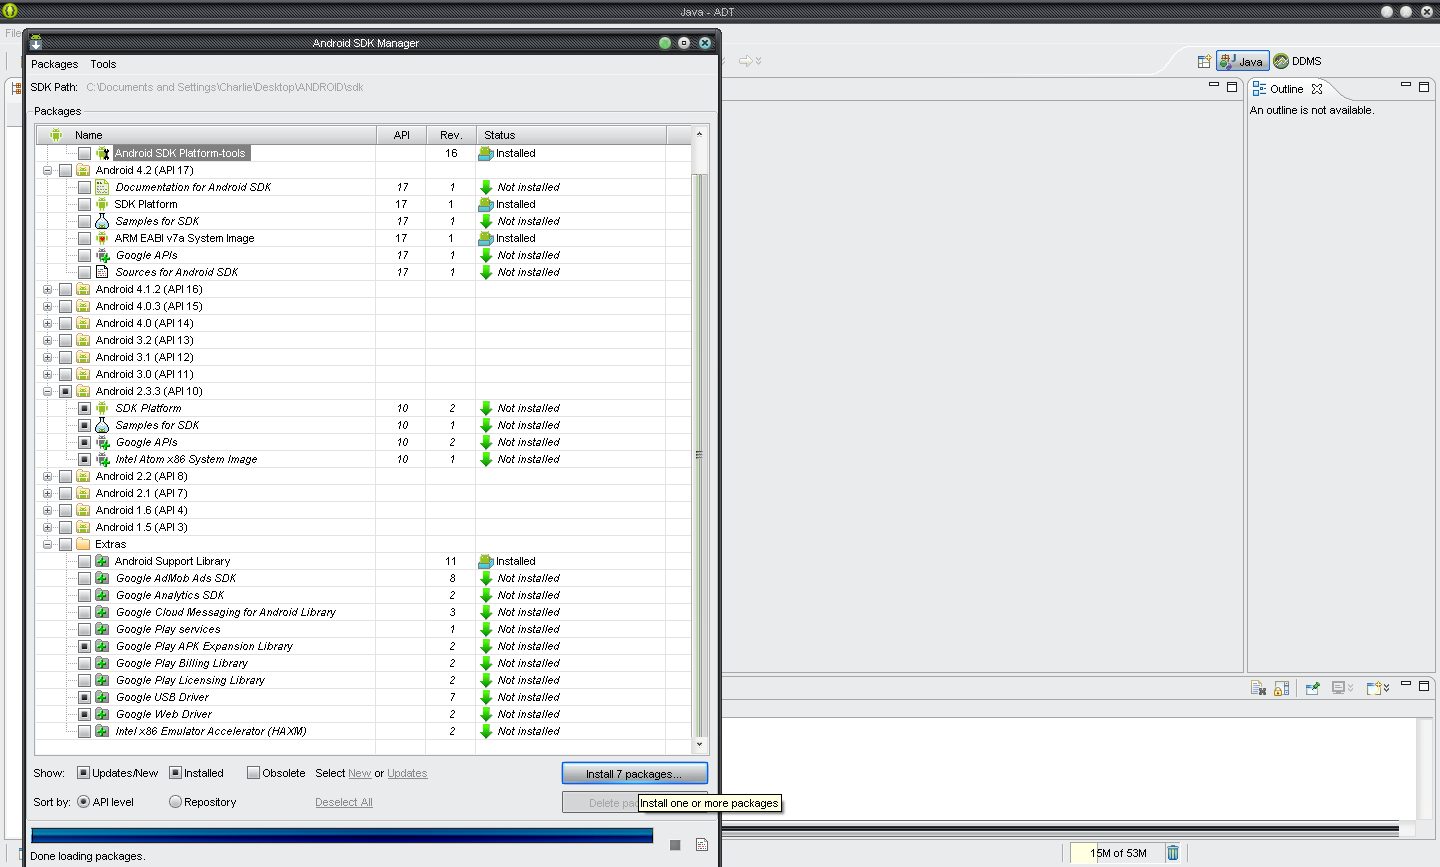
\includegraphics[width=1.0\textwidth]{tutorial_9}
  \caption{Términos de contrato}
  \label{fig:tutorial_9}
\end{figure}
\end{enumerate}

\newpage
\section{Hola mundo y el simulador de Android}

Primero que nada un fragmento del código para el hola mundo, de ahora en adelante cada vez que hablemos de una actividad mostraremos dos partes del código el .xml correspondiente a la interfaz y el código Java correspondiente a la actividad, hay que tener especial cuidado cuando se programa para Android pues los nombres de los objetos de la interfaz como lo son los campos de texto y los botones deben ser muy dicientes pues estos se pueden llegar a confundir o refundir entre más grande sea la aplicación, la explicación es la siguiente:

La parte XML:

\begin{itemize}
\item RelativeLayout: Clase para representar un cuadro de contenido cuyas margenes y elementos se definen por como se posicionan unos al lado de otros.
\item TextView: Clase que sirve para representar un campo de texto, es el equivalente a Label en Java.
	\begin{itemize}
	\item id: Identificador del cuadro de texto.
	\item layout width: Ancho del cuadro de texto, algunas opciones son:
		\begin{itemize}
		\item match parent: Forma automática de acomodar el tamaño usando como referencia el contenedor.
		\item wrap content: Forma automática de acomodar el tamaño usando como referencia el contenido cercano al objeto.
		\item fill parent: Forma automática de acomodar el tamaño llenando por completo el contenedor.
		\end{itemize}
	\item layout height: Alto del cuadro de texto.
	\item centerHorizontal: Aclarar si se centra respecto al contenedor de forma horizontal.
	\item centerVertical: Aclarar si se centra respecto al contenedor de forma vertical.
	\item text: texto a mostrar, normalmente todas las cadenas se almacenan en @string el cual se encuentra configurado en res/values/strings.xml.
	\end{itemize}
\end{itemize}

\begin{lstlisting}
<RelativeLayout xmlns:android="http://schemas.android.com/apk/res/android"
    xmlns:tools="http://schemas.android.com/tools"
    android:layout_width="match_parent"
    android:layout_height="match_parent"
    tools:context=".MainActivity" >

    <TextView
        android:id="@+id/labelDeTexto"
        android:layout_width="wrap_content"
        android:layout_height="wrap_content"
        android:layout_centerHorizontal="true"
        android:layout_centerVertical="true"
        android:text="@string/hello_world" />

</RelativeLayout>
\end{lstlisting}

La parte JAVA:

\begin{itemize}
\item Bundle: Clase que sirve para transmitir tipos primarios de datos a través de las actividades.
\item Activity: Clase que representa una actividad de Android, se puede interpretar como cada pantalla o servicio que se provee en la aplicación.
\item Menu: Toda actividad trae un menú al cual se le puede agregar opciones modificando el xml o directamente en la clase.
\item TextView: Clase que sirve para representar un campo de texto, es el equivalente a Label en Java.
\item setContentView(): Método que define la interfaz que sera usada por esta actividad.
\item findViewById(): Método que encuentra una vista u objeto como el cuadro de texto que definimos en el xml, R hace referencia a un codigo autogenerado donde se encuentran todos los recursos.
\end{itemize}
\newpage
\begin{lstlisting}
//HolaMundo.java
package com.example.ejemplo1;

import android.os.Bundle;
import android.app.Activity;
import android.view.Menu;
import android.widget.TextView;

public class MainActivity extends Activity {
	
    TextView labelDeTexto;

    @Override
    public void onCreate(Bundle savedInstanceState) {
        super.onCreate(savedInstanceState);
        setContentView(R.layout.activity_main);
        labelDeTexto = (TextView) findViewById(R.id.labelDeTexto);
        labelDeTexto.setText("Hola Mundo");
    }

    @Override
    public boolean onCreateOptionsMenu(Menu menu) {
        getMenuInflater().inflate(R.menu.activity_main, menu);
        return true;
    }
}

}

\end{lstlisting}
\section{Botones, textos y otros}
blablablabla

\chapter{Varias actividades una sola aplicación}              
blablablabla
\section{Intent y la secuencia de actividades}
blablablabla
\section{Layout orden en el caos}
blablablabla
\section{Vistas y más vistas}
blablablabla
\section{Fechas y contactos}
blablablabla
\section{Tabs, menús y preferencias}
blablablabla

\chapter{Código avanzado}              
blablablabla
\section{SQLite y archivos planos}
blablablabla
\section{Cambios de orientación}
blablablabla
\section{Estilos e imagen}
blablablabla
\section{Permisos y conexiones}
blablablabla

\chapter{Sensores}
blablablabla              
\section{Rotación y brújulas}
blablablabla
\section{GPS}
blablablabla
\section{Archivos}
blablablabla


\part{Interacción con Android}  

\chapter{Java y Android}
blablablabla              
\section{Aplicaciones Java de Escritorio}
blablablabla
\section{Tipos de datos compartidos}
blablablabla
\section{Exportación y conexión}
blablablabla                 



%index
%\newpage
%\addcontentsline{toc}{chapter}{Index}
%\printindex


%glossary
\newpage
\printglossary

\end{document}                          % The required last line
